\documentclass[letterpaper,journal]{IEEEtran}
\usepackage{amsmath,amsfonts}
\usepackage{algorithmic}
\usepackage{algorithm}
\usepackage{array}
\usepackage[caption=false,font=normalsize,labelfont=sf,textfont=sf]{subfig}
\usepackage{textcomp}
\usepackage{stfloats}
\usepackage{url}
\usepackage{verbatim}
\usepackage{graphicx}
\usepackage{cite}
\usepackage{booktabs}

\usepackage{amssymb}

\hyphenation{op-tical net-works semi-conduc-tor IEEE-Xplore}
% updated with editorial comments 8/9/2021

\begin{document}

\title{EMERGE: Evolutionary Memory-Augmented Multi-Agent Reasoning for Multi-Robot Task Allocation}

\author{IEEE Publication Technology,~\IEEEmembership{Staff,~IEEE,}
        % <-this % stops a space
\thanks{For videos and prompting details, please visit our project website: https://
sites.google.com/andrew.cmu.edu/llmcraft/home.}% <-this % stops a space
\thanks{Manuscript received April 19, 2021; revised August 16, 2021.}}

% The paper headers
\markboth{Journal of \LaTeX\ Class Files,~Vol.~14, No.~8, August~2021}%
{Shell \MakeLowercase{\textit{et al.}}: A Sample Article Using IEEEtran.cls for IEEE Journals}

\IEEEpubid{0000--0000/00\$00.00~\copyright~2021 IEEE}
% Remember, if you use this you must call \IEEEpubidadjcol in the second
% column for its text to clear the IEEEpubid mark.

\maketitle

\begin{abstract}
Large language models (LLMs) have shown promising reasoning capabilities for robotic planning and decision-making. However, existing LLM-based robotic systems often solve each task instance in isolation, limiting their ability to transfer prior task-solving experience across related problem settings. This limitation is particularly critical in multi-robot task allocation (MRTA), where diverse allocation problems often share reusable structural patterns while differing in task multiplicity, robot requirements, temporal constraints, and coordination forms. This paper proposes EMERGE, an evolutionary memory-augmented multi-agent reasoning framework for MRTA. Given a natural-language MRTA problem description, EMERGE generates an executable solver and returns the corresponding robot-task allocation result through structured stages of task understanding, problem formulation, and solver generation. It further introduces an explicit evolutionary memory mechanism that organizes, retrieves, and refines historical task-solving experience, enabling the system to reuse and adapt prior knowledge when solving new MRTA instances. We construct a benchmark covering eight canonical MRTA settings, including single-task and multi-task, single-robot and multi-robot, and instantaneous and time-extended allocation scenarios. Simulation and real-robot experiments show that EMERGE consistently outperforms existing LLM-based baselines, achieving stronger cross-setting generalization and better allocation performance across diverse MRTA problems.

\end{abstract}

\begin{IEEEkeywords}
Large language models, Task allocation, Memory, benchmark.
\end{IEEEkeywords}

\section{Introduction}

\IEEEPARstart{M}{ulti}-robot systems (MRS) have been widely adopted in real-world applications due to their robustness, scalability, and ability to accomplish complex tasks through cooperation~\cite{verma2021multi,li2025large}. A central challenge in MRS is multi-robot task allocation (MRTA), which determines how tasks should be assigned to robots under diverse task requirements, robot capabilities, temporal constraints, and coordination structures\cite{chakraa2023optimization}. Recently, large language models (LLMs) have shown promise for MRTA by providing strong semantic understanding and reasoning capabilities, especially when task specifications are expressed in natural language\cite{yu2025clga}. However, existing LLM-based MRTA methods still tend to solve each new task instance in isolation. As a result, they often fail to explicitly organize and reuse prior task-solving experience, making it difficult to transfer historical knowledge to new allocation settings even when different tasks share similar underlying structures.



\begin{figure}[!t]
  \centering
  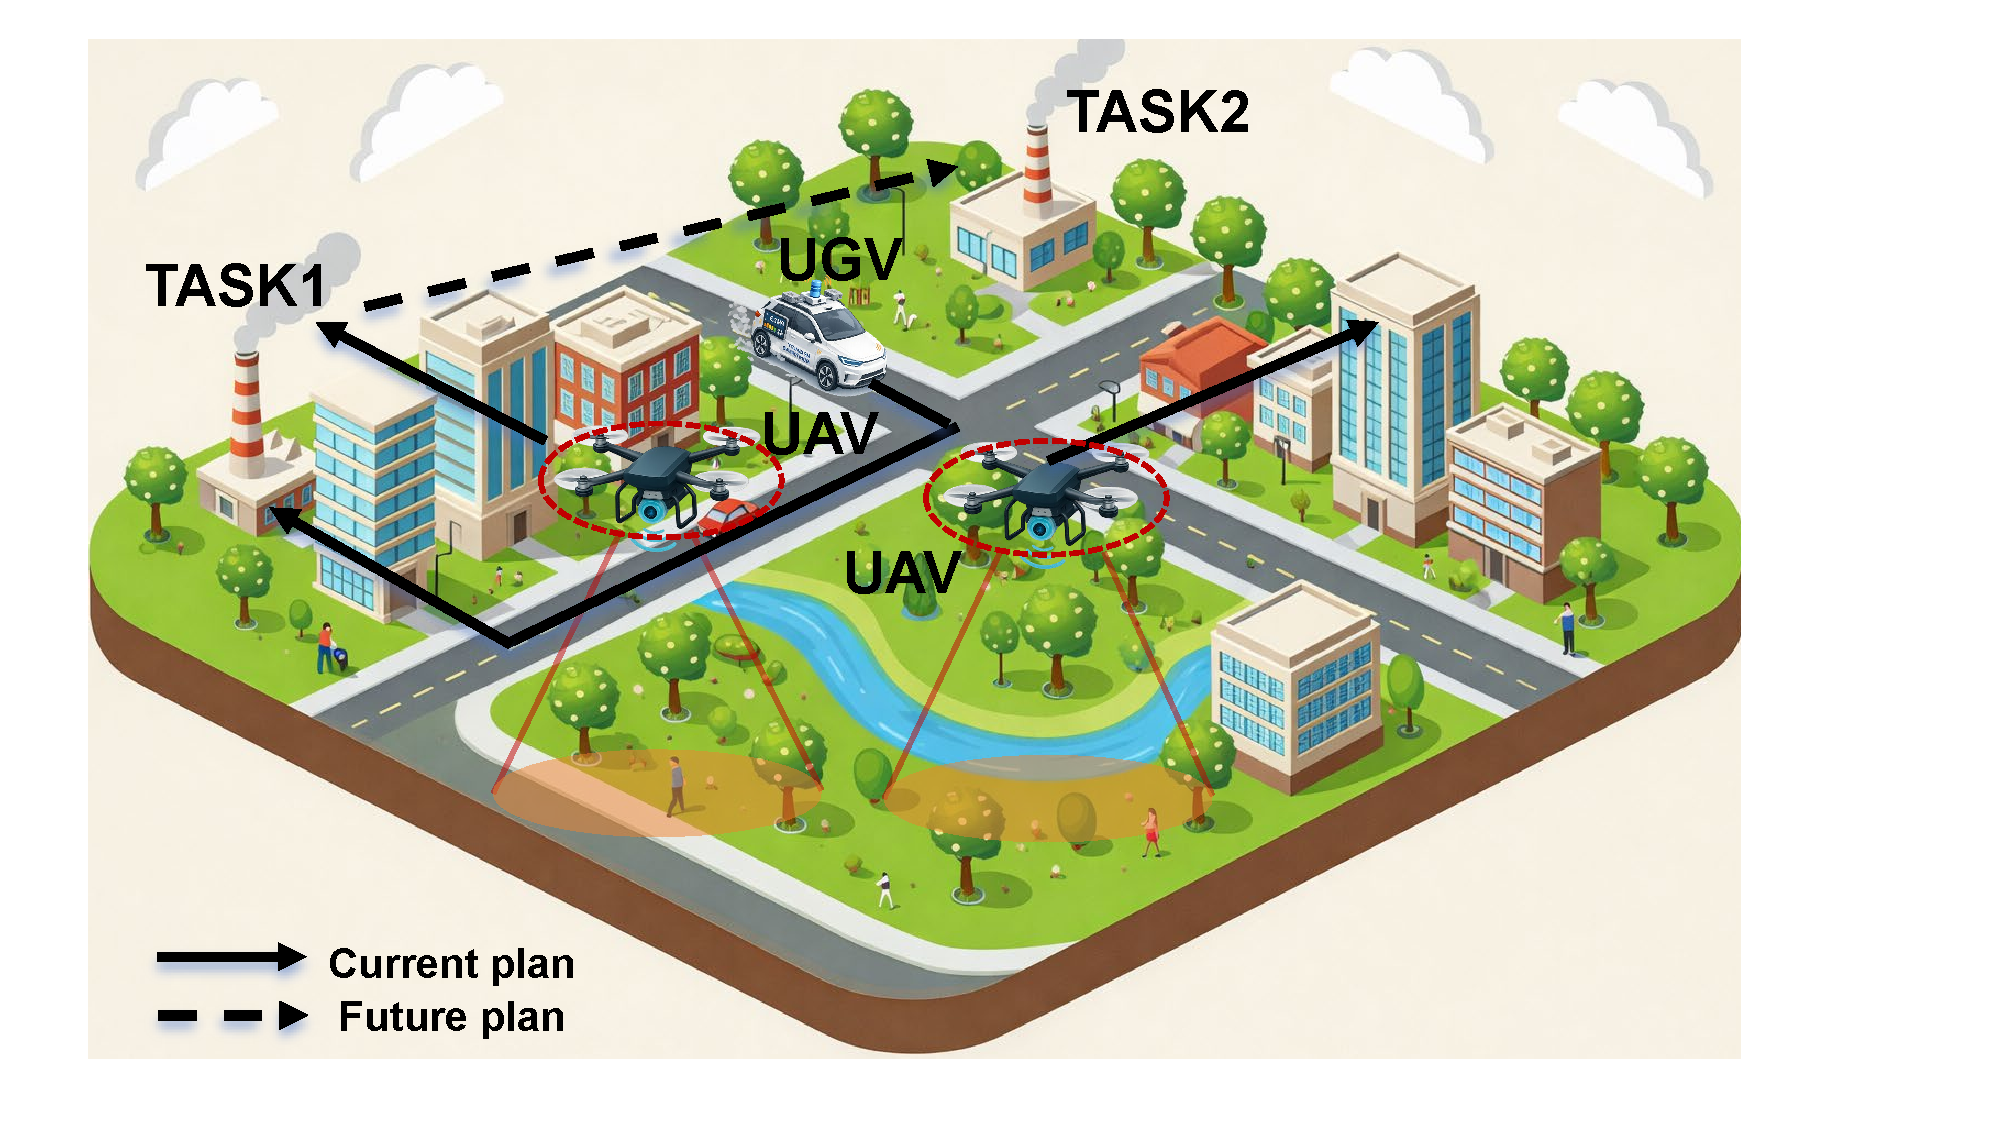
\includegraphics[width=0.9\columnwidth]{figure/fig1.pdf}
  \caption{In pollution monitoring and mitigation, UAVs may first inspect suspected regions, after which UGVs are assigned to mitigation tasks under capability, precedence, and time-window constraints. Although such a mission differs semantically from warehouse delivery or search-and-rescue, it may share reusable allocation knowledge at different abstraction levels. }
  \label{fig1}
\end{figure}

Existing LLM-based multi-robot planning methods can be broadly divided into two categories. The first uses LLMs as auxiliary modules for task understanding, instruction parsing, or high-level plan generation, while final allocation and coordination decisions are handled by conventional planners or optimization-based solvers\cite{yu2025clga}. The second places LLMs directly in the decision-making loop to generate task decompositions or allocation decisions\cite{kannan2024smart}. Despite their differences, both categories largely rely on per-instance reasoning and provide limited support for accumulating reusable allocation experience. This limitation is particularly critical for MRTA, where structurally related problems may differ in task multiplicity, robot requirements, temporal extension, and coordination forms, but still share reusable modeling and solving patterns. Moreover, existing studies are often evaluated on ad-hoc or task-specific scenarios, lacking systematic benchmarks that capture the structural diversity of MRTA and support principled evaluation of cross-setting generalization~\cite{yu2025clga,kannan2024smart}. Without such a benchmark, it remains difficult to determine whether an LLM-based MRTA method truly learns transferable allocation patterns or only performs well on a narrow set of hand-crafted scenarios.

\IEEEpubidadjcol
To address these limitations, we propose EMERGE, an evolutionary memory-augmented multi-agent reasoning framework for MRTA. In this work, we focus on natural-language MRTA solving, where the input is a textual task description and the desired output is a valid robot-task allocation. EMERGE decomposes MRTA solving into a structured multi-agent reasoning process, where specialized agents collaboratively perform task understanding, problem formulation, and solver generation. Built on this reasoning process, EMERGE introduces a dual-layer evolutionary memory mechanism to organize historical task-solving experience at both the instance and abstract levels. Instance-level memories preserve fine-grained task-specific experiences, including task formulations, solver patterns, execution feedback, and allocation results, enabling the reuse of concrete experience for similar task instances. Abstract memories maintain category-level summaries that capture reusable modeling regularities and corrective knowledge beyond individual cases. Execution feedback is used to update the memory repository, enabling the framework to refine previous MRTA solutions and transfer them to new task settings rather than treating each instance independently.

To systematically evaluate transfer across MRTA settings, we further construct a systematic MRTA benchmark with 200 natural-language problem instances spanning all eight canonical combinations of single-/multi-task robots, single-/multi-robot tasks, and instantaneous/time-extended allocation~\cite{korsah2013comprehensive}. This benchmark provides a unified testbed for evaluating whether LLM-based MRTA solvers can generalize across structurally different allocation settings. Extensive simulation and real-robot experiments demonstrate that EMERGE consistently outperforms existing LLM-based baselines, achieving stronger cross-setting generalization and more robust allocation performance across diverse task allocation scenarios.
The main contributions of this work are summarized as follows:
\begin{itemize}
    \item An evolutionary memory-augmented multi-agent reasoning framework, termed EMERGE, is proposed for transferable MRTA solving.
    \item A dual-layer evolutionary memory mechanism is designed to organize, retrieve, and refine historical task-solving experience.
    \item An eight-category MRTA benchmark is constructed, and simulation and real-robot experiments demonstrate the improved generalization of EMERGE.
\end{itemize}



\section{Related Work}

\subsection{Multi-Robot Task Allocation}
Multi-robot task allocation (MRTA) is a core problem in multi-robot systems, involving task coordination, distributed assignment, coalition formation, and cooperative execution~\cite{aziz2022task,antonyshyn2023multiple,faigl2012goal}. Existing MRTA methods are commonly developed under optimization-based, market-based, and learning-based paradigms. Optimization-based approaches formulate MRTA as combinatorial optimization problems and solve them with exact or approximate algorithms, such as matching-based formulations and Hungarian assignment~\cite{sung2020distributed}. Market-based methods allocate tasks through bidding or auction mechanisms, with consensus-based auction schemes as representative examples~\cite{lusk2020distributed,choi2009consensus}. Learning-based methods infer allocation policies or robot-task compatibility from data, including graph-neural-network models over robot-task bipartite graphs~\cite{liu2024glan}. Although effective in specific settings, these methods typically rely on predefined formulations or instance-wise solving pipelines, with limited support for organizing prior solutions as reusable experience across heterogeneous MRTA settings.

\subsection{LLM-Based Planning for Multi-Robot Systems}
LLMs have recently been introduced into robotic and multi-robot planning due to their semantic understanding and reasoning capabilities. Existing methods either use LLMs as auxiliary modules for task understanding, instruction parsing, or high-level plan generation, while leaving allocation and coordination to conventional planners or solvers, or directly place LLMs in the decision-making loop to generate task decompositions, coalition structures, or allocation decisions~\cite{huang2022language,di2023towards,liu2023llm+,cao2023robot,vemprala2024chatgpt,huang2023inner,kannan2024smart}. Despite improved flexibility, most methods still solve allocation problems on a per-instance basis, with limited mechanisms for accumulating and reusing historical task-solving experience. Moreover, existing evaluations are often task-specific, making it difficult to systematically assess cross-setting generalization and memory-based adaptation.

\subsection{Memory-Augmented Reasoning and Transfer Evaluation}


Memory mechanisms have been investigated in natural language processing and language-agent systems, where they are mainly used to retrieve external knowledge, maintain interaction histories, or accumulate reusable skills for long-horizon reasoning and tool use~\cite{zhong2024memorybank,wang2025agent,xu2026mem}. In robotics, memory has also been used to support long-horizon perception and control, for example by maintaining spatial-temporal context or past interaction experience.~\cite{anwar2025remembr,yang2023neural}. Nevertheless, existing memory mechanisms have rarely been designed for MRTA. Unlike language or control tasks, MRTA requires memory to encode structured allocation experience, including task formulations, robot-task coupling, allocation constraints, solver programs, generated schedules, and execution-aware feedback. Such experience must be abstracted and reused at the task-category level to support transfer across MRTA settings.


\begin{figure*}[thpb]
  \centering
  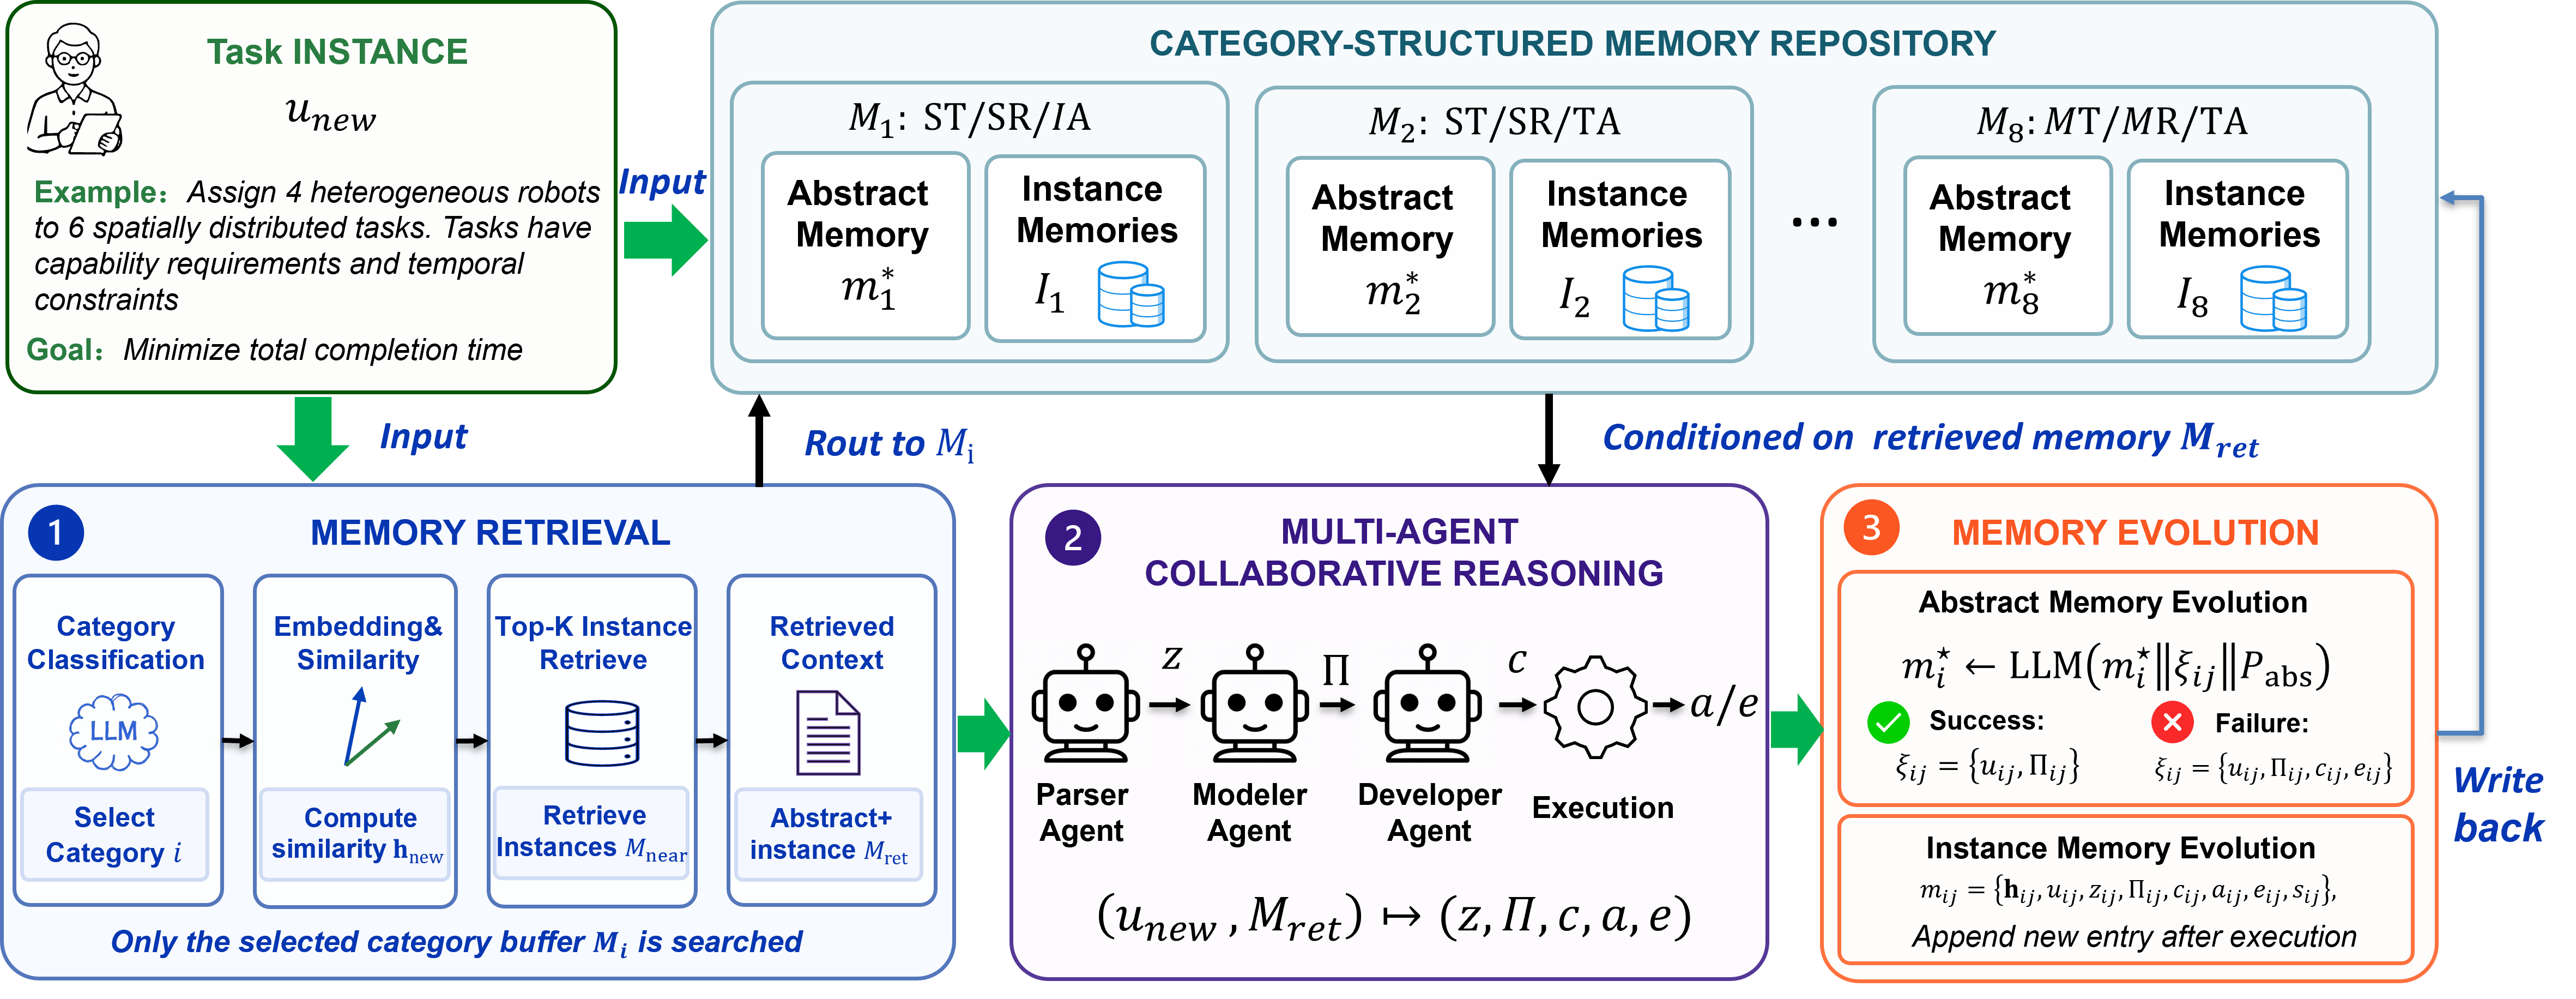
\includegraphics[width=18cm]{figure/framework.png}
  \caption{Overview of EMERGE, an evolutionary memory-augmented multi-agent reasoning framework for transferable MRTA solving.}
  \label{fig2}
\end{figure*}



\section{Method}

EMERGE solves natural-language MRTA problems by generating executable solver programs and executing them to obtain allocation solutions, with historical task-solving experience reused through evolutionary memory.

\subsection{Overview and Problem Setup}
Given a newly provided natural-language MRTA task description \(u_{\mathrm{new}}\) and a memory repository \(\mathcal{M}\), EMERGE aims to generate an executable solver and obtain solver outputs together with execution feedback. The overall process is formulated as
\begin{equation}
(u_{\mathrm{new}},\mathcal{M}) \mapsto (z,\Pi,c,a,e),
\end{equation}
where \(z\) is the structured task representation extracted from \(u_{\mathrm{new}}\), \(\Pi\) is the instantiated MRTA optimization problem, \(c\) is the generated executable solver program, \(a\) is the resulting solution, and \(e\) is the execution feedback returned after solver execution. 
The memory repository \(\mathcal{M}\) is queried before reasoning to provide reusable experience and is updated after execution using the newly generated task-solving record. In the online solving process, EMERGE first routes \(u_{\mathrm{new}}\) to an MRTA category, retrieves a category-specific memory context \(M_{\mathrm{ret}}\) from the memory repository \(\mathcal{M}\), performs memory-conditioned collaborative reasoning, and finally updates the corresponding memory buffer using the generated task-solving record.






\subsection{Multi-Agent Collaborative Reasoning}


Conditioned on the retrieved memory context \(M_{\mathrm{ret}}\), EMERGE uses three specialized reasoning agents to solve an MRTA problem: a Parser \(\mathcal{A}_{\mathrm{Par}}\), a Modeler \(\mathcal{A}_{\mathrm{Mod}}\), and a Developer \(\mathcal{A}_{\mathrm{Dev}}\). These agents are responsible for task parsing, optimization modeling, and solver synthesis, respectively. They are instantiated with different role-specific prompts:
\[
\mathcal{A}_{r}(x \mid C;P_r),
\quad r\in\{\mathrm{Par},\mathrm{Mod},\mathrm{Dev}\},
\]
where \(x\) denotes the current input, \(C\) denotes the accumulated context including retrieved memory and previous agent comments, and \(P_r\) denotes the role-specific prompt. After each agent produces its output, the output is stored as an intermediate comment and becomes part of the context for subsequent agents. 





\subsubsection{Parser}
The Parser is responsible for task parsing and schema induction for MRTA. Rather than merely interpreting the task description at the semantic level, it extracts the core structural elements required for optimization-oriented reasoning, including the robot set, the task set, and the schema-level decision structure implied by the input. Formally, the Parser maps the new task description \(u_{\mathrm{new}}\) to a structured representation
\begin{equation}
z=\mathcal{A}_{\mathrm{Par}}(u_{\mathrm{new}}\mid M_{\mathrm{ret}};P_{\mathrm{Par}}).
\end{equation}
where \(\mathcal{A}_{\mathrm{Par}}\) denotes the Parser agent conditioned on the retrieved memory context \(M_{\mathrm{ret}}\). The resulting representation
\[
z = (\mathcal{R}, \mathcal{T}, \mathcal{D})
\]
captures the structural entities of the MRTA problem, where 
\(\mathcal{R}=\{r_n\}_{n=1}^{N_R}\) denotes the available robots with their capability attributes, 
\(\mathcal{T}=\{\tau_\ell\}_{\ell=1}^{N_T}\) denotes the tasks with their requirements and execution conditions, and \(\mathcal{D}\) denotes the decision schema induced by the MRTA category, including whether each robot can execute single or multiple tasks, whether each task requires single or multiple robots, and whether the allocation is instantaneous or time-extended.



\subsubsection{Modeler}
The Modeler \(\mathcal{A}_{\mathrm{Mod}}\) transforms the structured representation \(z\) into a concrete mathematical optimization problem. Since \(z\) encodes the optimization-relevant entities and decision schema extracted from the original task description, the Modeler determines appropriate objectives, variables, and constraints, and instantiates them according to the task structure. Formally, this process can be written as
\begin{equation}
\Pi=\mathcal{A}_{\mathrm{Mod}}(u_{\mathrm{new}},z\mid M_{\mathrm{ret}};P_{\mathrm{Mod}}),
\end{equation}
where \(\Pi\) denotes the instantiated MRTA optimization problem, expressed in the generic form
\begin{equation}
\Pi:\quad
\min_{x\in\mathcal{X}}\; \mathcal{O}(x;z)
\quad \text{s.t.} \quad
g_q(x;z)\le 0,\; q=1,\dots,Q,
\end{equation}
where \(x\) denotes the concrete optimization variables instantiated from the decision schema \(\mathcal{D}\), \(\mathcal{X}\) denotes the corresponding feasible domain, \(\mathcal{O}(x;z)\) is the task-dependent objective function, and \(g_q(x;z)\) represents the \(q\)-th task-dependent constraint. Depending on the task category, \(\Pi\) may take the form of an assignment, coalition-formation, scheduling, routing, or coupled optimization model. The formulation is output in \LaTeX\ format to ensure interpretability and to facilitate subsequent solver code generation.


\subsubsection{Developer}
The Developer \(\mathcal{A}_{\mathrm{Dev}}\) translates the formal MRTA optimization problem into an executable optimization program. Given the instantiated optimization problem \(\Pi\), it generates solver code that implements decision-variable declaration, objective construction, constraint encoding, and solver invocation in a machine-executable form. Formally, the Developer produces
\begin{equation}
c=\mathcal{A}_{\mathrm{Dev}}(u_{\mathrm{new}},z,\Pi\mid M_{\mathrm{ret}};P_{\mathrm{Dev}}).
\end{equation}
where \(c\) denotes an executable solver program and \(M_{\mathrm{ret}}\) provides retrieved implementation guidance, such as previously successful solver templates or coding patterns. In our implementation, the Developer generates Python code using Gurobi~\cite{gurobi} as the optimization backend. Although our implementation uses Python with Gurobi as the backend, the Developer only requires a machine-executable solver interface; thus the design is not tied to a specific optimizer. Executing \(c\) yields an allocation result and execution feedback, which can be written as $(a,e)=\mathrm{Exec}(c)$, where \(e\) may include solver status, infeasibility diagnostics, and runtime error messages. These outputs are later stored as part of the corresponding instance memory and used for memory evolution.


\subsection{Evolutionary Memory Mechanism}
Because MRTA instances differ not only in task semantics but also in allocation structure, a flat memory pool may mix incompatible modeling patterns. EMERGE therefore organizes memory according to the standard MRTA taxonomy based on three orthogonal dimensions, namely single- vs.\ multi-task robots (ST/MT), single- vs.\ multi-robot tasks (SR/MR), and instantaneous vs.\ time-extended allocation (IA/TA). This taxonomy induces eight canonical MRTA categories, based on which EMERGE organizes memory to capture both category-level regularities and instance-level reusable experience. In the following, we describe the evolutionary memory mechanism from three aspects: memory structure, memory retrieval, and memory evolution.




\subsubsection{Category-Structured Memory Repository}
To support experience accumulation across heterogeneous MRTA tasks, we organize memory into eight category-specific buffers rather than a single flat memory pool. Formally, the memory repository is defined as
\begin{equation}
\mathcal{M} = \{ M_1, M_2, \dots, M_8 \},
\end{equation}
where each \(M_i\) corresponds to one canonical MRTA category. Each category-specific memory adopts a dual-layer structure:
\begin{equation}
M_i = \{ m_i^{\star} \} \cup \mathcal{I}_i,
\end{equation}
where \(m_i^{\star}\) denotes the abstract memory for category \(i\), and \(\mathcal{I}_i\) denotes the corresponding set of instance memories. Hereafter, \(i\) indexes an MRTA category, and \(j\) indexes a historical task instance within category \(i\).

\subsubsection{Memory Retrieval}
Given the new task description \(u_{\mathrm{new}}\), memory retrieval is performed in two stages: category routing and within-category instance retrieval. In the category-routing stage, EMERGE first infers the MRTA category of \(u_{\mathrm{new}}\) as
\begin{equation}
i \leftarrow \mathrm{LLM}\bigl(u_{\mathrm{new}} ; P_{\mathrm{cls}}\bigr),
\end{equation}
where \(P_{\mathrm{cls}}\) is the category-classification prompt and \(i \in \{1,\dots,8\}\) denotes one of the eight canonical MRTA categories induced by the combinations of ST/MT, SR/MR, and IA/TA. The query is then routed to the corresponding category-specific memory \(M_i\). The second stage retrieves the most relevant instance memories within that buffer based on embedding similarity. The embedding of the new task is first computed as
\begin{equation}
\mathbf{h}_{\mathrm{new}} = f_{\mathrm{enc}}(u_{\mathrm{new}}).
\end{equation}
After determining its category \(i\), cosine similarity is computed between the new task and each instance memory in \(\mathcal{I}_i\):
\begin{equation}
\mathrm{Sim}_{ij} =
\frac{\mathbf{h}_{\mathrm{new}} \cdot \mathbf{h}_{ij}}
{\|\mathbf{h}_{\mathrm{new}}\| \|\mathbf{h}_{ij}\|}.
\end{equation}
Retrieval then selects the Top-\(K\) instance memories from \(\mathcal{I}_i\) according to their similarity scores:
\begin{equation}
M_{\mathrm{near}} =
\operatorname{TopK}_{m_{ij}\in\mathcal{I}_i}
\bigl(m_{ij}; \mathrm{Sim}_{ij}, K\bigr).
\end{equation}
Similarity-based retrieval is performed over the retained instance memories in $\mathcal{I}_i$. The retrieved memory context is constructed as
\begin{equation}
M_{\mathrm{ret}} = \{ m_i^{\star} \} \cup M_{\mathrm{near}} .
\end{equation}
The abstract memory \(m_i^{\star}\) provides category-level modeling guidance, whereas \(M_{\mathrm{near}}\) provides instance exemplars.


\subsubsection{Abstract Memory Evolution}

For each executed task instance \(j\) in category \(i\), the abstract memory \(m_i^{\star}\) is incrementally updated to capture reusable knowledge at the category level. We formulate abstract-memory evolution in a unified form as
\begin{equation}
m_i^{\star} \leftarrow \mathrm{LLM}\bigl(m_i^{\star} , \xi_{ij}; P_{\mathrm{abs}}\bigr),
\end{equation}
where \(\xi_{ij}\) denotes the update context constructed from the corresponding task-solving episode, and \(P_{\mathrm{abs}}\) denotes the abstraction prompt for category-level memory refinement. For a successful episode, \(\xi_{ij}\) contains the task description and the resulting optimization formulation, i.e., \(\xi_{ij}=\{u_{ij},\Pi_{ij}\}\), so that the abstract memory captures reusable category-level patterns in objectives, constraints, and decision-variable design. For a failed episode, \(\xi_{ij}\) additionally includes the generated solver program and execution feedback, i.e., \(\xi_{ij}=\{u_{ij},\Pi_{ij},c_{ij},e_{ij}\}\), enabling the abstract memory to accumulate corrective knowledge such as common failure modes, infeasibility causes, and useful modeling or implementation revisions. For successful episodes, we focus the abstract update on \(u_{ij}\) and \(\Pi_{ij}\), since the abstract memory is intended to summarize reusable modeling patterns rather than store full execution traces. Detailed solver code, allocation outputs, and feedback are preserved in the instance memory.



\subsubsection{Instance Memory Evolution}

The instance memory $\mathcal{I}_i$ represents a collection of instance entries whose size is bounded by the category-specific maximum capacity $N_i$. Each detailed memory entry is defined as
\begin{equation}
m_{ij} = \{ u_{ij}, \mathbf{h}_{ij}, z_{ij}, \Pi_{ij}, c_{ij}, a_{ij}, e_{ij}, s_{ij} \},
\end{equation}
where \(u_{ij}\) denotes the \(j\)-th historical task description in category \(i\), and \(\mathbf{h}_{ij}=f_{\mathrm{enc}}(u_{ij})\) is its embedding.
The symbolic task formulation \(z_{ij}\), the instantiated optimization problem \(\Pi_{ij}\), the generated solver program \(c_{ij}\), the allocation result \(a_{ij}\), and the execution feedback \(e_{ij}\) are produced during task execution. After execution, these outputs are consolidated into an instance memory entry \(m_{ij}\) and appended to the corresponding category buffer \(\mathcal{I}_i\). The access frequency \(s_{ij}\) is used for memory retention. For a newly added entry, the access frequency is initialized as \(s_{ij}=1\). The access frequency is incremented upon each retrieval, i.e., \(s_{ij} \leftarrow s_{ij} + 1\). In this work, we use access frequency as a simple retention criterion, while more advanced quality-, diversity-, or recency-aware memory management strategies can be incorporated into the same buffer structure.

\subsubsection{Implementation Details}
In our implementation, the three reasoning agents are instantiated using the same LLM backbone with different role-specific prompts. Task descriptions are encoded by a text embedding model for within-category memory retrieval. We encode each task description using the pre-trained sentence embedding model \texttt{all-MiniLM-L6-v2} from Sentence-Transformers~\cite{reimers2019sentencebert}, which maps text into 384-dimensional dense representations. The Developer generates Python programs with Gurobi as the optimization backend, while \(K\) and \(N_i\) control retrieval size and category-specific memory capacity, respectively.


\begin{algorithm}[t]
\caption{EMERGE Inference and Memory Evolution}
\label{alg:emerge}
\begin{algorithmic}[1]
\REQUIRE Task description $u_{\mathrm{new}}$, memory repository $\mathcal{M}$, retrieval size $K$, buffer capacity $N_i$
\ENSURE Allocation result $a_{\mathrm{new}}$, execution feedback $e_{\mathrm{new}}$, and updated memory repository $\mathcal{M}$
\STATE Infer the task category $i$ for $u_{\mathrm{new}}$.
\STATE Encode $u_{\mathrm{new}}$ as $\mathbf{h}_{\mathrm{new}}$.
\STATE Retrieve $M_{\mathrm{near}}$ as the Top-$K$ subset of $\mathcal{I}_i$ according to similarity scores.
\STATE Increment the access frequencies of the retrieved instance memories in $M_{\mathrm{near}}$.
\STATE Set $M_{\mathrm{ret}}=\{m_i^{\star}\}\cup M_{\mathrm{near}}$.
\STATE $z=\mathcal{A}_{\mathrm{Par}}(u_{\mathrm{new}}\mid M_{\mathrm{ret}};P_{\mathrm{Par}})$.
\STATE $\Pi=\mathcal{A}_{\mathrm{Mod}}(u_{\mathrm{new}},z\mid M_{\mathrm{ret}};P_{\mathrm{Mod}})$.
\STATE $c=\mathcal{A}_{\mathrm{Dev}}(u_{\mathrm{new}},z,\Pi\mid M_{\mathrm{ret}};P_{\mathrm{Dev}})$.
\STATE Execute $c$ to obtain an allocation result $a_{\mathrm{new}}$ (or $\varnothing$ if no valid allocation result is returned) and feedback $e_{\mathrm{new}}$.
\STATE Initialize the access frequency of the new memory entry as $s_{\mathrm{new}}=1$.
\STATE If $a_{\mathrm{new}}\neq \varnothing$, update $m_i^{\star}$ using $\{u_{\mathrm{new}},\Pi\}$; otherwise update $m_i^{\star}$ using $\{u_{\mathrm{new}},\Pi,c,e_{\mathrm{new}}\}$.
\STATE Store $m_{\mathrm{new}}=\{\mathbf{h}_{\mathrm{new}},u_{\mathrm{new}},z,\Pi,c,e_{\mathrm{new}},a_{\mathrm{new}},s_{\mathrm{new}}\}$ in $\mathcal{I}_i$.
\STATE If $|\mathcal{I}_i|>N_i$, retain the top $N_i$ entries in $\mathcal{I}_i$ by access frequency.
\RETURN $a_{\mathrm{new}}$, $e_{\mathrm{new}}$, and updated $\mathcal{M}$.
\end{algorithmic}
\end{algorithm}

\section{Experiment}
To evaluate the effectiveness and generalizability of EMERGE, we construct a taxonomy-driven MRTA benchmark covering eight canonical allocation categories. We then compare EMERGE with existing LLM-based methods and conduct analyses of task allocation quality, transferability to unseen categories and scenarios, ablation of key components, error patterns, and feasibility on a real-robot platform.



\subsection{Benchmark Construction}

We construct an MRTA benchmark based on the classical MRTA taxonomy with 200 instances~\cite{korsah2013comprehensive}. The taxonomy follows three binary dimensions: robot capability, including single-task (ST) and multi-task (MT) robots; task requirement, including single-robot (SR) and multi-robot (MR) tasks; and assignment temporality, including instantaneous assignment (IA) and time-extended assignment (TA). These three binary dimensions combine to form eight canonical MRTA categories, each containing 25 instances, including 10 scenario-agnostic instances and 15 scenario-specific instances. The scenario-agnostic instances describe generic MRTA structures without application-specific semantics, while the scenario-specific instances instantiate similar allocation structures in concrete domains, such as urban air-quality monitoring, traffic surveillance, power facility inspection, forest ecological monitoring, and large-event security coverage.


Each instance includes a natural-language problem description and a JSON test case with robot/task positions, capability assumptions, task requirements, temporal windows when applicable, and ground-truth outputs. Fig.~\ref{figexa} illustrates a representative MT/MR/TA benchmark instance. Panel (a) gives the natural-language description of an urban air-quality monitoring task with three drones, three pollution-sensing zones, and three time steps, highlighting the multi-task, multi-robot, and time-window constraints. Panel (b) provides the corresponding structured input/output, including robot and task positions, feasible execution steps, task requirements, and the ground-truth output. The objective is to minimize the total Euclidean travel distance while satisfying robot-task matching, collaboration, and time-window constraints.


\begin{figure}[!t]
  \centering
  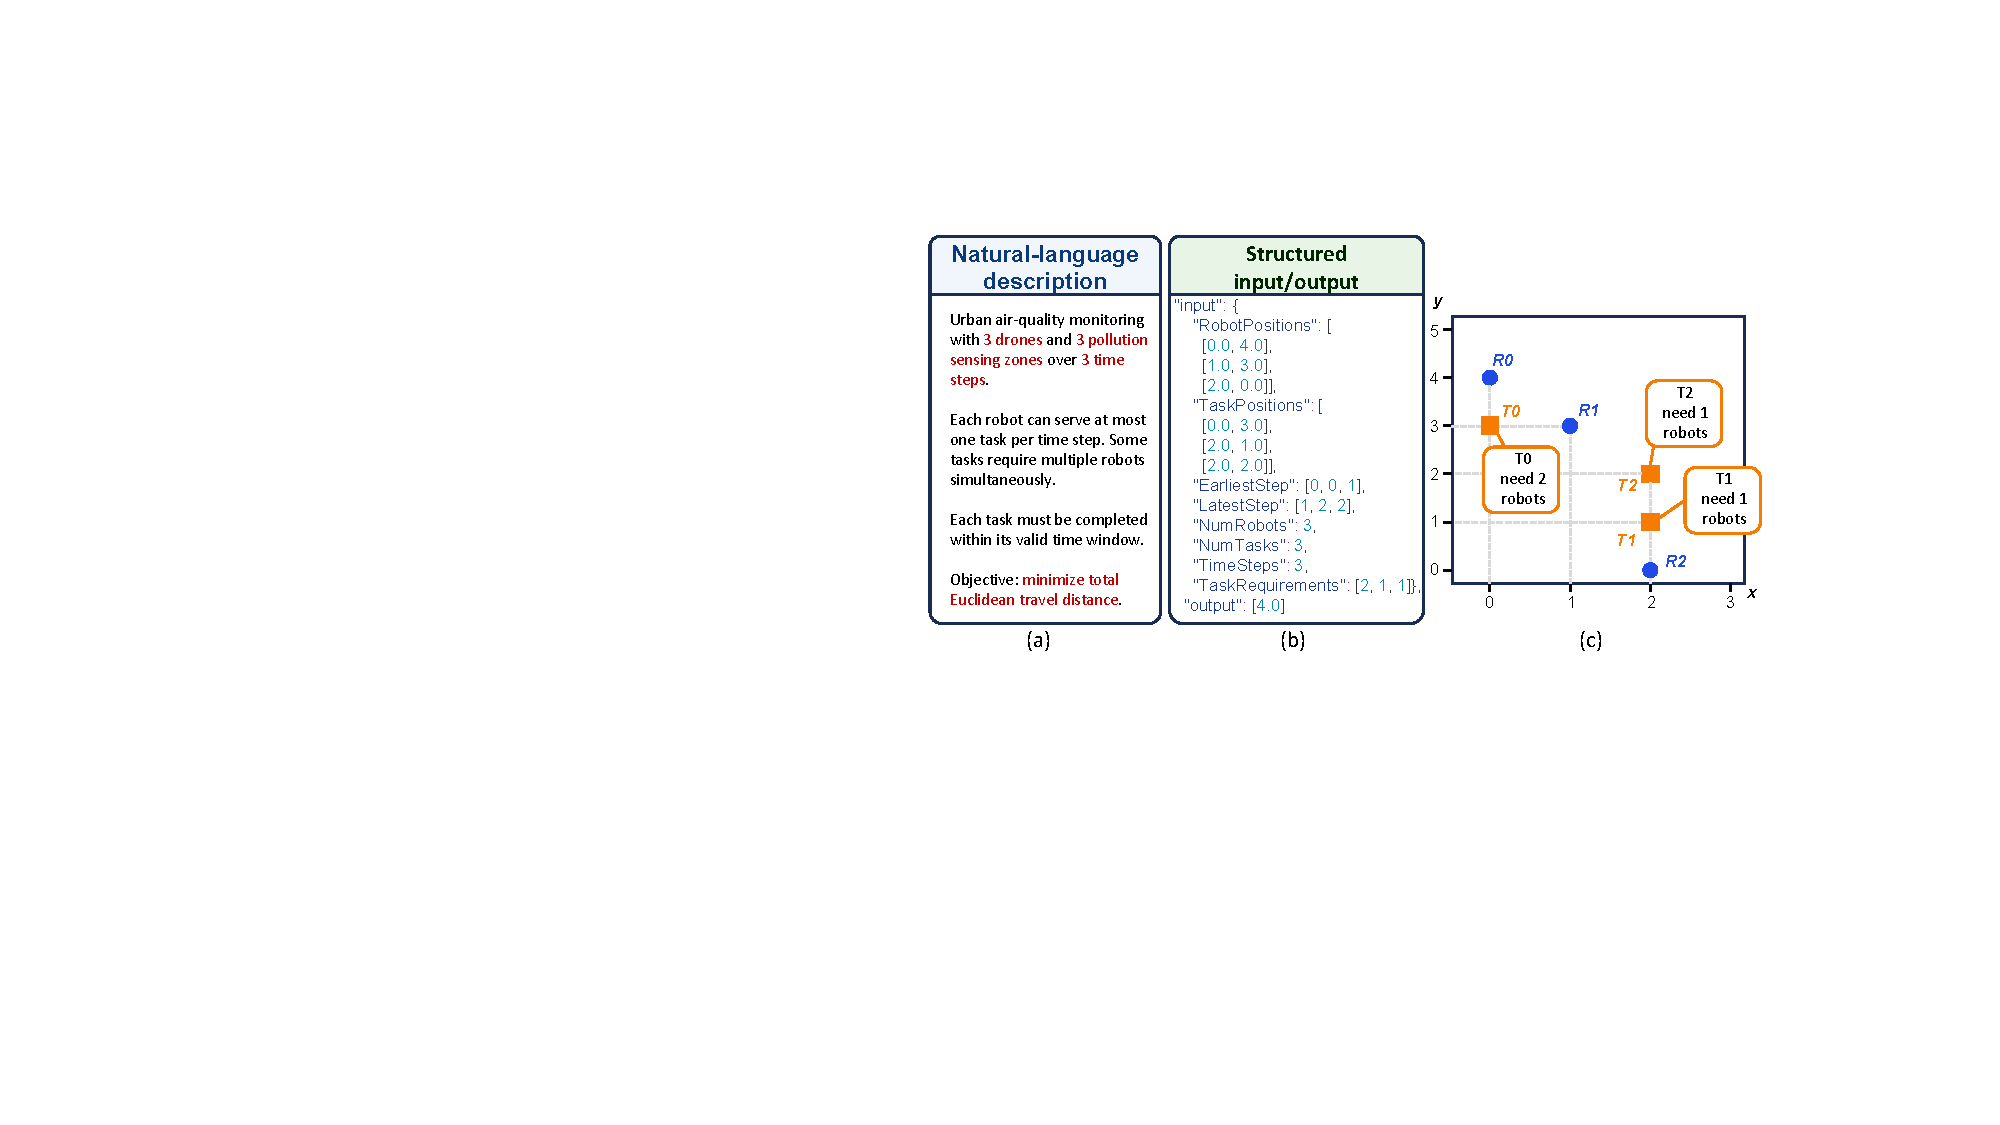
\includegraphics[width=0.9\columnwidth]{figure/example.pdf}
  \caption{Example MT/MR/TA instance from the proposed benchmark. (a) Simplified natural-language description. (b) JSON test case. (c) 2-D visualization of robot and task locations, task requirements, and feasible time windows.}
  \label{figexa}
\end{figure}

\subsection{Baseline}
We evaluate EMERGE on natural-language MRTA problems against four LLM-based baselines: PHP~\cite{PHP}, CLGA~\cite{yu2025clga}, CoT~\cite{wei2022chain}, and Standard. Standard directly prompts the LLM to generate executable code from the task description. For each instance in the benchmark, the generated program is executed and checked by an automatic evaluator. A trial is counted as successful only if the program runs correctly and returns an allocation that matches the ground truth while satisfying all constraints.


\subsection{Overall Performance}
\begin{table}[t]
\centering
\caption{Success rate (\%) comparison across different settings.}
\label{tab:success_rate_mtsr}
\begin{tabular}{lccccc}
\toprule
MRTA & \textbf{Ours} & CLGA & Standard & PHP &  COT \\
\midrule
MT/MR/IA & 100\% & 76\% & 72\% & 68\%   & 75\% \\
MT/MR/TA & 64\% & 48\% & 48\% & 36\%   & 32\% \\
MT/SR/IA & 96\% & 92\% & 92\% & 84\%   & 92\% \\
MT/SR/TA & 88\% & 36\% & 28\% & 36\%   & 28\% \\
ST/MR/IA & 100\% & 88\% & 84\% & 68\%   & 84\% \\
ST/MR/TA & 88\% & 80\% & 74\% & 72\%   & 76\% \\
ST/SR/IA & 100\% & 88\% & 84\% & 44\%   & 92\% \\
ST/SR/TA & 88\% & 64\% & 60\% & 64\%   & 64\% \\
\midrule
Overall  & 88.5\%  & 63.3\%  & 86\%  & 59\% &  70\% \\
\bottomrule
\end{tabular}
\end{table}

Table~\ref{tab:success_rate_mtsr} reports the success rates of different methods across the eight MRTA configurations. Overall, the proposed method achieves the highest average success rate of 87.5\%, outperforming all baseline approaches. Notably, our method maintains consistently strong performance across all MRTA categories, including the most challenging configurations involving multi-robot tasks and time-extended assignment. For instantaneous assignment (IA) problems, all methods perform relatively well on single-robot task settings (ST/SR/IA and MT/SR/IA), reflecting the limited structural complexity of these cases. However, in multi-robot task settings (ST/MR/IA and MT/MR/IA), our method consistently achieves near-perfect success rates, indicating its ability to effectively reason about coordination and coalition formation even in instantaneous decision scenarios. The performance gap becomes more pronounced in time-extended assignment (TA) problems, which require long-horizon planning and task sequencing.
In particular, for MT/MR/TA and MT/SR/TA settings, our method significantly outperforms all baselines, while chain-of-thought-based and optimization-driven methods exhibit substantial degradation.
This highlights the advantage of the proposed memory-augmented framework in handling temporal dependencies and cross-task coupling. Across all configurations, baseline methods tend to perform competitively in simpler ST/SR cases but show reduced robustness as task structures become more complex, especially when both multi-robot cooperation and temporal reasoning are required.
In contrast, the proposed approach demonstrates stable performance across all eight MRTA categories, supporting its effectiveness for transferable and structure-aware MRTA solving.

The category-wise results show that the benchmark is not merely a collection of instances, but a diagnostic testbed that exposes how different methods behave under increasing structural complexity, especially in time-extended and multi-robot settings.
% 体现benchmark的区分度
% 现在 success rate 表已经很有用，但你可以在分析中强调：这个 benchmark 不是只看 overall，而是能暴露不同 MRTA 子类的难度差异。比如 MT/MR/TA、MT/SR/TA 这类 time-extended 场景明显更难，基线下降更明显，而 EMERGE 更稳定。这能说明 benchmark 的价值不只是“多”，而是“有诊断能力”。
\begin{table}[htbp]
\centering
\caption{Cross-class and cross-scene generalization results across eight MRTA categories.}
\label{tab:mrta_cross_generalization}
\begin{tabular}{lccc}
\toprule
\textbf{Task Type} & \textbf{Cross-Class} & \textbf{Cross-Scene}   & \textbf{w/o Mem} \\
\midrule
MT/MR/IA & 96\%  & 92\%    & 100\% \\
MT/MR/TA & 40\%  & 80\%    & 0\% \\
MT/SR/IA & 88\%  & 100\%   & 92\% \\
MT/SR/TA & 32\%  & 60\%    & 4\% \\
ST/MR/IA & 88\%  & 100\%   & 100\%  \\
ST/MR/TA & 84\%  & 80\%    & 76\% \\
ST/SR/IA & 100\% & 86.67\% & 100\%  \\
ST/SR/TA & 76\%  & 80\%    & 68\%   \\
\bottomrule
\end{tabular}
\end{table}



\subsection{Transferability Analysis}
\label{sec}

We design two transfer experiments to evaluate whether the memory in EMERGE can be reused across different MRTA structures and application scenarios.

\textbf{Cross-category transfer.} For each target MRTA category, we first run EMERGE on all non-target categories to update its abstract memory with solving experience from other MRTA structures. We then evaluate EMERGE on the target category, where only the abstract memory from non-target categories is retrieved and no instance-level memory from the target category is used. As reported in Table~\ref{tab:mrta_cross_generalization}, EMERGE maintains reasonable performance, but the degradation is more evident in time-extended and multi-robot categories, where temporal reasoning and cooperative constraints are harder to transfer from abstract summaries alone.

\textbf{Cross-scenario transfer.} For each category, we first run EMERGE on the scenario-agnostic instances to update its memory with generic MRTA solving experience. We then evaluate it on the scenario-specific instances within the same category. The results show consistently higher performance than cross-category transfer, suggesting that generic MRTA solving experience can be effectively reused when the underlying allocation structure is shared across scenarios.

Overall, these results indicate that abstract memory captures transferable structural knowledge, while scenario-level adaptation further benefits from shared task formulations.



\begin{table}[t]
\centering
\footnotesize
\caption{Ablation Results Across MRTA Settings (\%)}
\label{tab:ablation_mrta}
\begin{tabular*}{\columnwidth}{@{\extracolsep{\fill}}lccccc@{}}
\toprule
\textbf{Task} 
& \textbf{w/o Mem} 
& \textbf{w/o Evo} 
& \textbf{w/o Forget} 
& \textbf{w/o Corr} 
& \textbf{Ours} \\
\midrule
MT/MR/IA & 100\% & 88\% & 84\% & 83.33\% & 100\% \\
MT/MR/TA & 12\%   & 12\% & 68\% & 41.67\% & 80\%  \\
MT/SR/IA & 92\%  & 52\% & 72\% & 84\%    & 88\%  \\
MT/SR/TA & 12\%   & 72\% & 76\% & 36\%    & 84\%  \\
ST/MR/IA & 100\% & 72\% & 96\% & 76\%    & 100\% \\
ST/MR/TA & 76\%  & 64\% & 56\% & 58.33\% & 88\%  \\
ST/SR/IA & 100\% & 76\% & 92\% & 88\%    & 100\% \\
ST/SR/TA & 68\%  & 52\% & 52\% & 56\%    & 88\%  \\
\midrule
\textbf{Overall} 
& 70\% 
& 61\% 
& 74.5\% 
& 65.42\% 
& \textbf{91\%} \\
\bottomrule
\end{tabular*}
\end{table}




\begin{table*}[t]
\centering
\footnotesize
\setlength{\tabcolsep}{3pt}
\caption{Success rate (\%) comparison across different MRTA categories.}
\label{tab:llm_mrta_results}
\begin{tabular}{lccccccccc}
\toprule
Model & MT-MR-IA & MT-MR-TA & MT-SR-IA & MT-SR-TA & ST-MR-IA & ST-MR-TA & ST-SR-IA & ST-SR-TA & Overall \\
\midrule
DeepSeek-V3 & 100\% & 64\% & 88\% & 84\% & 100\% & 88\% & 100\% & 88\% & 89\% \\
Claude-3.5 & 100\% & 70\% & 100\% & 30\% & 100\% & 100\% & 100\% & 40\% & 80\% \\
Gemini-2.5-F & 100\% & 90\% & 70\% & 50\% & 100\% & 70\% & 100\% & 80\% & 82.5\% \\
Gemini-2.5-P & 100\% & 90\% & 70\% & 100\% & 100\% & 80\% & 100\% & 50\% & 86.25\% \\
GPT-4o & 90\% & 10\% & 50\% & 50\% & 100\% & 90\% & 100\% & 100\% & 73.75\% \\
DeepSeek-V2.5 & 80\% & 50\% & 80\% & 70\% & 100\% & 90\% & 100\% & 100\% & 83.75\% \\
Qwen2.5-VL & 100\% & 60\% & 60\% & 50\% & 100\% & 90\% & 100\% & 90\% & 81.25\% \\
\bottomrule
\end{tabular}
\end{table*}



\subsection{Ablation Study}
Table~\ref{tab:ablation_mrta} reports the ablation results across the eight MRTA configurations.
The complete model achieves the best overall performance, indicating that all components contribute to the effectiveness of the proposed framework. Removing the memory module (w/o Mem) consistently degrades performance, with the most evident impact observed in time-extended assignment settings.
This suggests that explicit memory is important for reasoning over task sequences and maintaining consistency across longer planning horizons. When memory evolution is disabled (w/o Evo), performance drops across multiple configurations, implying that static memory alone is insufficient to support robust generalization across different MRTA structures. Similarly, removing access-frequency-based retention (w/o Forget) leads to reduced performance in several cases, indicating that retaining frequently accessed memories helps maintain memory relevance. Finally, excluding the self-correction mechanism (w/o Corr) results in a moderate but consistent decline across most settings, highlighting the role of iterative refinement in improving solution reliability. Overall, the ablation study demonstrates that the proposed components are complementary: memory enables structured reasoning, evolutionary updates support adaptation, access-frequency-based retention maintains robustness, and self-correction improves solution quality.





\subsection{Different LLM base models.} 
We evaluate the proposed MRTA framework under different LLM backbones to examine its robustness with respect to the choice of base model. The comparative results across multiple LLMs, including DeepSeek-V2.5, DeepSeek-V3, GPT-4o, Gemini-2.5 (Flash and Pro), Claude-3.5, and Qwen2.5-VL, are reported in Table~\ref{tab:llm_mrta_results}. Although the overall success rates differ among base models, each model solves a considerable portion of the eight MRTA configurations, indicating that the framework is not tied to a particular LLM. This suggests that the performance improvement mainly comes from the structured multi-agent reasoning process and the evolutionary memory mechanism, while stronger base models further enhance solving reliability and overall success rates.


\subsection{Analysis.} 
Figure \ref{venn} further analyzes the solved-instance overlap between EMERGE and the strongest baseline across the eight benchmark categories. EMERGE solves more instances in seven out of eight categories, with particularly large gains on MT/SR/TA and MT/MR/TA. The results show that the proposed benchmark exposes different levels of task difficulty, while EMERGE provides additional coverage beyond the baseline, especially in more challenging multi-task settings.

We further analyze the failure cases by categorizing each error according to its earliest failure source. As shown in Figure \ref{dis}, EMERGE reduces the total number of errors from 57 to 24 over 200 benchmark instances, achieving a 57.9\% relative reduction. The largest improvements occur in optimization objective errors and constraint condition errors, which decrease from 11 to 1 and from 24 to 7, respectively. This demonstrates that EMERGE primarily improves high-level MRTA formulation, including objective identification and constraint construction. Meanwhile, syntax errors only decrease slightly from 15 to 14, indicating that low-level coding mistakes remain partly limited by the base LLM's code generation ability.



\begin{figure}[!t]
  \centering
  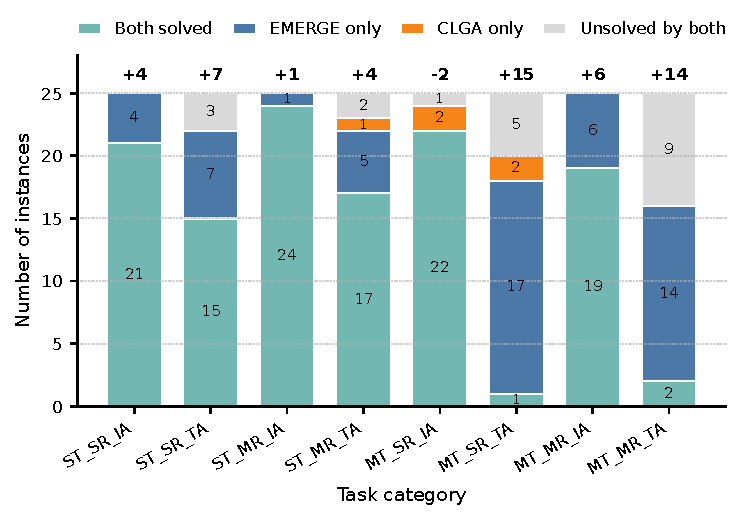
\includegraphics[width=0.9\columnwidth]{figure/venn_overlap.pdf}
  \caption{Solved-instance overlap across the eight categories. Each bar represents 25 instances from one task category. The stacked segments indicate instances solved by both methods, solved only by EMERGE, solved only by the strongest baseline, and unsolved by both methods. The numbers above the bars denote the net solved-instance gain of EMERGE over the baseline. }
  \label{venn}
\end{figure}

\begin{figure}[!t]
  \centering
  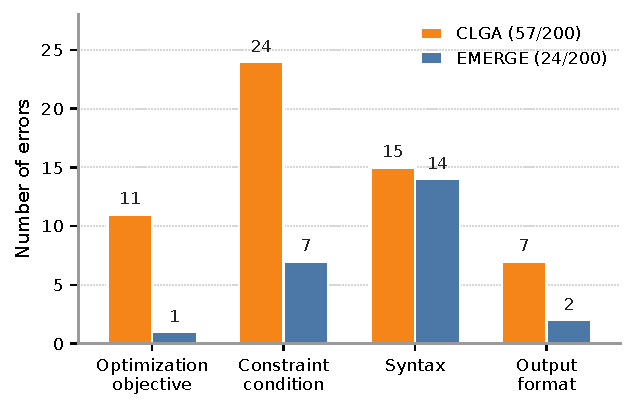
\includegraphics[width=0.9\columnwidth]{figure/error_distribution.pdf}
  \caption{Error-type distribution over 200 benchmark instances.
EMERGE substantially reduces formulation-related errors, especially in optimization objectives and constraint conditions.}
  \label{dis}
\end{figure}



\begin{figure}[!t]
  \centering
  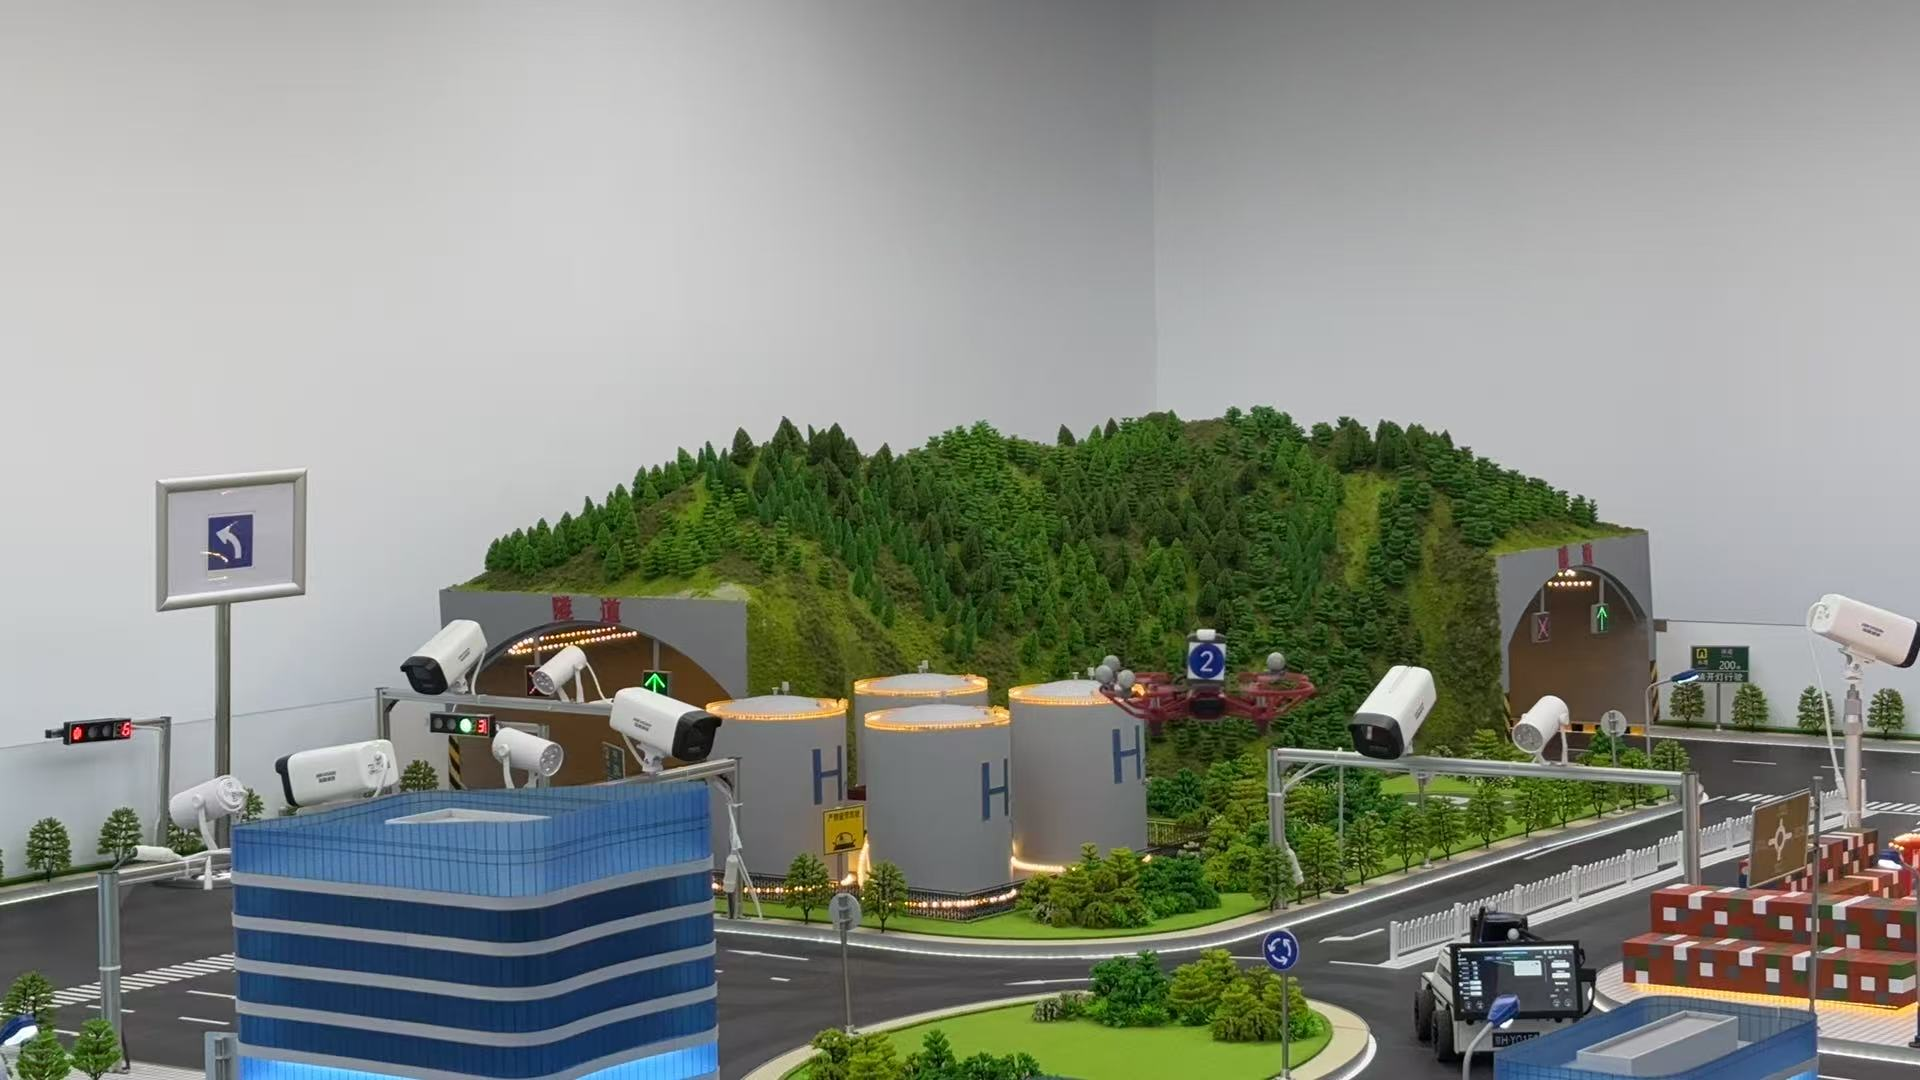
\includegraphics[width=0.9\columnwidth]{figure/phy.jpg}
  \caption{Cooperative pollution monitoring and mitigation with heterogeneous robots. Vectors denote robot capabilities and task requirements. UAVs perform pollution sensing, followed by UGVs executing mitigation actions. Arrows indicate robot schedules.}
  \label{fig_phy}
\end{figure}






\begin{table}[t]
\centering
\caption{Real-world robot experiment results.}
\label{tab:real_world}
\begin{tabular}{lcc}
\hline
\textbf{Scenario} & \textbf{Completion Success} & \textbf{Execution Time (s)} \\
\hline
Scenario 1 &  &  \\
Scenario 2 &  &  \\
\hline
\end{tabular}
\end{table}
\section{Conclusion}
In this work, we presented EMERGE, a memory-augmented multi-agent LLM framework for transferable MRTA solving. EMERGE integrates collaborative reasoning with a dual-layer evolutionary memory, allowing agents to reuse past experience across heterogeneous task structures rather than solving each task in isolation. Through specialized reasoning agents and execution-driven memory evolution, EMERGE handles diverse MRTA configurations. Experiments across eight canonical MRTA categories demonstrate its effectiveness across problem structures, scenarios, and LLM backbones without parameter fine-tuning of the underlying LLM. Cross-class and cross-scene evaluations further show that the evolved memories encode transferable structural knowledge, while ablation studies verify the complementary roles of memory construction, evolution, retention, and self-correction.




\bibliographystyle{IEEEtran}
\bibliography{ref}



\end{document}
